%%%%%%%%%%%%%%%%%%%%%%%%%%%%%%%%%%%%%%%%%%%%%%%%%%%%
\chapter{Inductance Characterization}\label{Appendix: AA}
\section{Inductance Estimation Table}



\section{Equivalent coil impedance} \label{AppendixSection: impedance}






%%%%%%%%%%%%%%%%%%%%%%%%%%%%%%%%%%%%%%%%%%%%%%%%%%%%
%%%%%%%%%%%%%%%%%%%%%%%%%%%%%%%%%%%%%%%%%%%%%%%%%%%%
%%%%%%%%%%%%%%%%%%%%%%%%%%%%%%%%%%%%%%%%%%%%%%%%%%%%
%%%%%%%%%%%%%%%%%%%%%%%%%%%%%%%%%%%%%%%%%%%%%%%%%%%%
\chapter{Model equations} \label{Appendix: A}
\section{Secondary capacitor in series} \label{sec:secondaryS}



\section{Secondary capacitor in parallel}\label{sec:secondaryP}

The same steps as above are followed for obtaining the impedances $Z_2$ and $Z_R$ when the secondary capacitor is placed in parallel: 


%%%%%%%%%%%%%%%%%%%%%%%%%%%%%%%%%%%%%%%%%%%%%%%%%%%%
%%%%%%%%%%%%%%%%%%%%%%%%%%%%%%%%%%%%%%%%%%%%%%%%%%%%
%%%%%%%%%%%%%%%%%%%%%%%%%%%%%%%%%%%%%%%%%%%%%%%%%%%%







%%%%%%%%%%%%%%%%%%%%%%%%%%%%%%%%%%%%%%%%%%%%%%%%%%%%
\chapter{Coils Experimental Results}
\section{Inductance and Resistance}\label{sec:RL}




\section{Quality Factor}








%%%%%%%%%%%%%%%%%%%%%%%%%%%%%%%%%%%%%%%%%%%%%%%%%%%%
%%%%%%%%%%%%%%%%%%%%%%%%%%%%%%%%%%%%%%%%%%%%%%%%%%%%
\chapter{Circuit Schematics}

\section{Voltage Regulator}\label{Appendix: DC-DC}

% \begin{figure}[htb]
% 	\begin{center}
% 		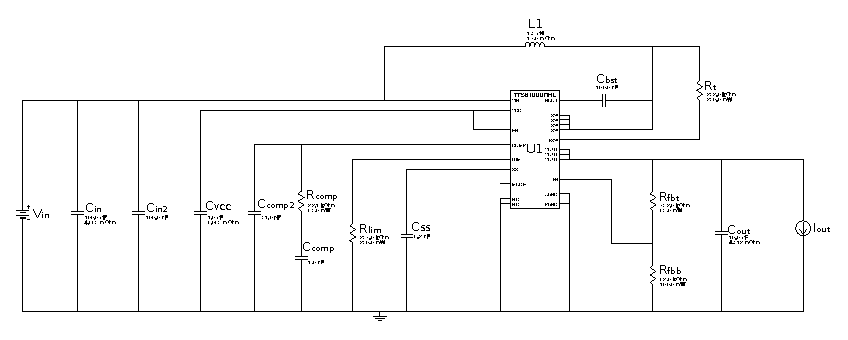
\includegraphics[width=1.05\textwidth]{./images/TPS61088}
% 	\caption{TPS61088 design circuit}
% 	\end{center}
% \end{figure}

